
\section{Labs}

\subsection{General}
What is the BTnode?
\begin{itemize}[noitemsep]
\item autonomous wireless communication and computing platform
\item has bluetooth radio
\item developed @eth
\item Atmel ATmega128L microcontroller, 8MHz, 64+180 KB RAM
\end{itemize}

Features
\begin{itemize}[noitemsep]
\item Non preemptive multi-threading
\item Events
\item Periodic and one-shot timers
\item Dynamic heap memory allocation
\item Interrupt driven streaming I/O
\end{itemize}


\subsection{Terminal/minicom}
We can connect to the BTnode by entering \grqq minicom usb0\grqq\ into the linux terminal. The following commands are then available:
\begin{itemize}[noitemsep]
\item bt - bluetooth radio
\item led - toggle LED patterns
\item bat - battery status
\item nut - show OS information
\item log - BTnut logging features
\end{itemize}

\subsection{Running Time}
In cycles, note: 8MHz cpu. \\
\begin{tabular}{|c|c|}
\hline brne (taken) & 2 \\ 
\hline brne (not taken) & 1 \\ 
\hline ldi & 1 \\ 
\hline rcall & 3 \\ 
\hline ret & 4 \\ 
\hline subi & 1 \\ 
\hline 
\end{tabular}

\subsection{Looping}
\begin{lstlisting}[basicstyle=\tiny]
//because only 8bit registers are available
//runs ca. 1.02 seconds
void waitabit() {
	int i, j;
	for(i = 0; i <= 1200; i++) {
		for(j = 0; j <= 1200; j++) {
			asm volatile  ("nop" ::);
		}
	}
}
\end{lstlisting}


\subsection{LED on}

\begin{lstlisting}[basicstyle=\tiny] %, %or \tiny ,\small or \footnotesize etc.

#include <avr/io.h>
void init(void) {
	MCUCR |= 1<<SRE; // enable external memory bus
	DDRB |= 1<<DDB5; // set latch pin as output
}
int main(void)
{
	volatile char* pointer;
	char dummy;
	init();
	// compute the pseudo-address that
	// contains the values for the LEDs
	//write 0x0 to turn off
	pointer  = (char*) (((short)0x2) << 8); //blue
	// force the compiler to write this
	// pseudo-address to the address-bus
	dummy   = * pointer;
	// now enable the latch
	PORTB |= 1<<PB5;
	// wait a moment - volatile keeps the
	// compiler from removing this line
	asm volatile  ("nop" ::);
	// disable the latch, i.e. hold the value
	PORTB &= ~(1<<PB5);
	return 0;
}

\end{lstlisting}

\subsection{Battery}


\subsubsection{Theorem}
We need a conversion from the input to get the voltage: $ ADC = \lceil 1023*V_in / V_ref \rceil$ with $V_ref = 3.3V$ Note, that this BAT-SENSE signal delivers the half voltage. For example, for 1V, then $\lceil 1023*0.5 / 3.3 \rceil = 155 $.

\subsubsection{Code}

To read out the battery value, we have to code the following: 

\begin{lstlisting}[basicstyle=\small]
ADCSRA |= 1<<ADPS0; //for the
ADCSRA |= 1<<ADPS1; // slowest
ADCSRA |= 1<<ADPS2; //speed = hightes accuracy
ADCSRA |= 1<<ADEN; // ADC enable to enable the ADC
ADCSRA |= 1<<ADSC; // ADC start conversion bit 
\end{lstlisting}

Do now a polling on the ADSC to check if conversion has finished. If so, read out the 10 bits (ADCL the lowest 8 bit, then ADCH the highest two bits).

\begin{tnote}
See Lab 2, Task 1.3 for the solution Code!
\end{tnote}

\subsection{Interrupts}
The interrupts are based on the ATmega128's Timer/Counter3. It has a Timer/Counter interrupt mask register (ETIMSK).
Because CPU as a frequency of 7.3 MHz, to generate a 2second timer, we compute: $2^{16} = 65536 clocks = 9ms$. So to get 2s, we compute $2s/9ms = 222.2$. So we take 256 as a prescalar and check, if the value reaches then $7.3Mhz/256*2s = 57031 = 0xdec7$.

\begin{lstlisting}[basicstyle=\small]
CR3AH = 0xde; //first part of the threshold (because only 8 bit)
CRAL = 0xc7; //second part of the threshold
ETIMSK |= 1 << OCIE3A; // interrupt is based on the threshold
\end{lstlisting}

The routine to register a interrupt has the following declaration: \texttt{NutRegisterIrgHandler(irq, handler, arg)}. Where
\begin{itemize}[noitemsep]
\item IRQ: Interrupt number to be associated with this handler. Zb \texttt{ sig\_OVERFLOW3} to register an overflow of counter3, \texttt {sig\_OUTPUT\_COMPARE3A} to trigger an interrupt if the counter reaches the threshold saved.
\item Handler: This routine is called by the OS, when a specified interrupt occurs
\item Arg: the argument passed
\end{itemize}

\begin{tnote}
See Lab 2, Task 2.2, 2.3 for the code
\end{tnote}

\subsection{OS}

\subsubsection{General}

\begin{itemize}[noitemsep]
\item Called Nut/OS
\item Three layers:
		\begin{itemize}
		\item the rudimentary C-libraries as implemented by avr-gcc’s $avr-libc$
		\item the higher-level OS routines built on top of $avr-libc$ by Nut/OS
		\item The BTnode-specific device drivers
		\end{itemize}
\item Compiled by avr-gcc
\item Compiled in the console by \texttt{ make btnode3 upload }
\item Main should never exit, otherwise the behaviour is undefined
\end{itemize}

\subsubsection{LED}
Light all four LEDS after each other.
\begin{lstlisting}[basicstyle=\small]
#include <hardware/btn-hardware.h>     /*for hardware init*/
#include <led/btn-led.h>               /*for LEDs*/
#include <sys/timer.h>                 /*for NutSleep*/
int main(void)
{
	u_char led = 0;
	btn_hardware_init();               /*init hardware*/
	btn_led_init(0);                   /*init LEDs*/
	for(;;)
	{
		led = 0;
		while (led < 4)
		{
			/*turn LED on*/
			btn_led_set(led);
			/*delay to make LED switch visible*/
			NutSleep(500);
			 /*turn LED off*/
			btn_led_clear(led);
			led++;
		}
	}
}
\end{lstlisting}


\subsubsection{Timer}

\begin{lstlisting}[basicstyle=\small]
#include <hardware/btn-hardware.h>
#include <sys/timer.h>
// use multiple timer if you have multiple methods to call
HANDLE hTimer; 
//arbitrary name for callback method
static void _tm_callback(HANDLE h, void* a)
{
	// do something when timer expires
}
int main (void)
{
	btn_hardware_init();
	//install and start timer
	//ARGS: a) time in ms (every 3 seconds)
	// b) Argument to pass
	//c) TM_ONESHOT (fire only once ) or 0 (periodic)
	
	hTimer = NutTimerStart(3000, _tm_callback, NULL, 0);
	for (;;) { NutSleep(1000); }
}

\end{lstlisting}

\subsubsection{Terminal}
On the host, run \texttt{ minicom usb0} or \texttt{ minicom usb1}. Check, if configured to \texttt{57.6k, 8N1, no flow control}.
\begin{tnote}
printf does not support \%f !
\end{tnote}

\begin{lstlisting}[basicstyle=\small]
#include <stdio.h>
#include <dev/usartavr.h>
//link the printf output
void init_stdout(void)
{
	u_long baud = 57600;
	NutRegisterDevice(&APP_UART, 0, 0);
	//r+ for read+write
	freopen(APP_UART.dev_name, "r+", stdout);
	_ioctl(_fileno(stdout), UART_SETSPEED, &baud);
}

int main(void)
{
	btn_hardware_init();
	init_stdout();

	int variable = 13;
	printf("Hello world, ");
	printf("my lucky number is %d\n",variable);
	for (;;);
}

\end{lstlisting}

\subsubsection{Threads}

\begin{itemize}[noitemsep]
\item Uses cooperative multithreading
\item Thread functions should never return. They are exited by themselves by explicitly calling \texttt{NutThreadExit();}
\item A thread can be in one of the following states: \texttt{RUNNING} (only one thread), \texttt {READY}, \texttt{SLEEPING}.
\item \texttt{NutThreadYield();} will check for threads that are more important than myself. If so, then another thread is run, otherwise it will keep running. It passes the current thread into the READY state.
\item Idle-Thread is a thread with lowest priority. Runs if no other thread can be run
\item \texttt{NutSleep(INTEGER\_TIME\_IN\_MS); } will set the thread into the \texttt{SLEEPING} state and run another thread that is waiting (or the idle-thread)
\item There are priorities. Can be set with \texttt{NutThreadSetPriority(INTEGER);}. 0 is hightes priority, 254 lowest priority! Default is 64
\item Waiting for an event puts the thread into the \texttt{SLEEPING} state.
\item Multiple threads with the same priority are executed in FIFO order
\item A thread can get his name by using \texttt{ runningThread->td\_name}
\end{itemize}


Because of the higher priority, the thread my\_thread will not give up the cpu.
\begin{lstlisting}[basicstyle=\small]
#include <hardware/btn-hardware.h>
#include <sys/thread.h>
#include <led/btn-led.h>

// without any NutThreadYield the red LED is on
THREAD(my_thread, arg)
{
	//higher priority: red is on
	NutThreadSetPriority(20);
	
	// lower priority: blue is on
	//NutThreadSetPriority(80);
	for(;;)
	{
		btn_led_set(LED0);
		btn_led_clear(LED1);
		NutThreadYield();
	}
}
int main(void)
{
	btn_hardware_init();
	btn_led_init(0);
	NutThreadCreate("My thread", my_thread, 0, 192);
	for(;;)
	{
		btn_led_clear(LED0);
		btn_led_set(LED1);
		NutThreadYield();
	}
}
\end{lstlisting}


\subsubsection{Events}
\begin{itemize}[noitemsep]
\item Datatype \texttt {HANDLE var\_name }
\item Post an event by \texttt{NutEventPost(\&event) }
\item Wait for an event by \texttt { NutEventWait(\&event, timeout)}. For infinite timeout, use \texttt {NUT\_WAIT\_INFINITE}
\end{itemize}

\begin{tnote}
See Lab 3, Task 6 for code.
\end{tnote}


\section{Bluetooth}

\subsection{Overview}

\begin{figure}[ht]
	\centering
  	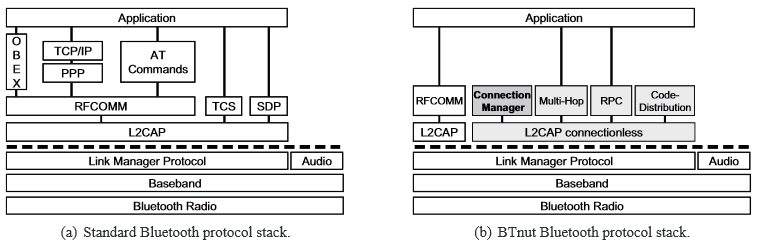
\includegraphics[scale=0.5]{img/lab_bluetooth_overview.png}
	\caption{Comparison between the the standard and the BTnut Bluetooth protocol stack}
	\label{fig_bluetooth_overview}
\end{figure}

\begin{itemize}[noitemsep]
\item Link Manager Protocol (LMP): controls the radio link between two devices.
\item Host Controller Interface (HCI): defines a common standardized interface between the Bluetooth host (e.g. the Atmega128 microcontroller) and the Bluetooth controller (e.g. the baseband controller and the Bluetooth radio)
\item Logical Link Control and Adaptation Protocol (L2CAP): provides an abstract interface for data communication
\item Connection Manager: forms and maintains a connected topology, manages discovery and connection of devices.
\item Multi-Hop: performs multi-hop routing and forwarding, provides an API for sending and receiving packets.
\end{itemize}


\subsection{Bluetooth Header}
\begin{itemize}
\item Byte [0, 4]: HCI-header
\item Byte [5, 8]: L2CAP header
\item Byte [5, 6]: message length. To set the length, use \texttt{ packet[HCI\_HEADER\_LEN] = (char) (msg\_len \& 0xFF) } and  \texttt{packet[HCI\_HEADER\_LEN + 1] = (char) ((msg\_len >> 8) \& 0xFF)}. To read the length, use \texttt{int msg\_len = packet[5] | (packet[6] << 8);}
\item Byte [7, 8]: channel. To set the channel, use \texttt{packet[HCI\_HEADER\_LEN + 2] = (char) (CHANNEL \& 0xFF);} and \texttt{packet[HCI\_HEADER\_LEN + 3] = (char) ((CHANNEL >> 8) \& 0xFF);}
\item Byte [9, ...]: The message
\end{itemize}


\section{Threads}

\subsection{Creating a thread}

\begin{lstlisting}[basicstyle=\tiny]
THREAD(my_thread, arg)
{
	for(;;)
	{ //do something }
}

int main(void)
{
	//192 = stack size
	if( 0 == NutThreadCreate("My thread", my_thread, 0, 192)) 
	{ //creation failed }
	
	for(;;)
	{ //do something }
}
\end{lstlisting}


\subsection{Terminating a thread}

\begin{lstlisting}[basicstyle=\tiny]
THREAD(my_thread, arg)
{
	for(;;)
	{ //do something 
	
		//can only kill itself
		if( CONDITION )
			NutThreadExit();
	}
}
\end{lstlisting}


\subsection{Sleep}


\begin{lstlisting}[basicstyle=\tiny]
THREAD(my_thread, arg)
{
	for(;;)
	{
		//do something 
		NutSleep(1000);
	}
}
\end{lstlisting}

\subsection{Co-Operative Scheduling}


\begin{lstlisting}[basicstyle=\tiny]
#include <sys/event.h>

HANDLE my_event;

THREAD(thread_A, arg)
{
	for(;;)
	{
		//do something 
		NutEventWait(&my_event, NUT_WAIT_INFINITE);
		//do something
	}
}

THREAD(thread_B, arg)
{
	for(;;)
	{
		//do something
		NutEventPost(&my_event);
		//so something
	}
}
\end{lstlisting}



\cleardoublepage
